\input ../SlidePreamble
\input ../preamble

\begin{document}

{\Huge

  \centerline{\bf TTIC 31230, Fundamentals of Deep Learning}
  \bigskip
  \centerline{David McAllester, Winter 2019}
  \vfill
  \centerline{\bf Language Modeling}
  \vfill
  \centerline{\bf Machine Translation}
  \vfill
  \centerline{\bf Attention}
  \vfill
  \centerline{\bf Beam Search}
  \vfill
  \centerline{\bf Error-Based Training}

\slide{Digression on Tensor Notation}

We will assume a high level RNN procedure $\mathrm{RNN}_\Phi$ which takes a sequence of input vectors and returns
a sequence of hidden state vectors.

\vfill
$$h[T,J] = \mathrm{RNN}_\Phi(x[T,I])$$

\vfill
Here, and in the future, we use capital letter indeces to denote tensors and lower case indeces to denote particular values from tensors.

\vfill
We will also omit the batch index.  Minibatching can be viewed as an efficiency optimization.

\slide{Digression on Tensor Notation}

We use capital letter indeces to denote tensors and lower case indeces to denote particular values from tensors.

\vfill
The equation
$$\tilde{L}[\ell+1,j] = \left(\sum_i\;W[\ell,i,j]L[\ell,i]\right) + \beta[\ell,j]$$
stands for a set of assignments --- one for each value $\ell$ and $j$

\slide{Slicing Notation}

A mixture of upper and lower case indeces denotes a slice.

\vfill
$h[t,J]$ denotes the vector whose $j$th component is $h[t,j]$.

\vfill
$L[X,Y,j]$ denotes the matrix (image) determined by the $j$th channel.

\slide{}


\centerline{\bf Different Forms of RNN}
\vfill
\vfill


\slide{Basic RNN}

\centerline{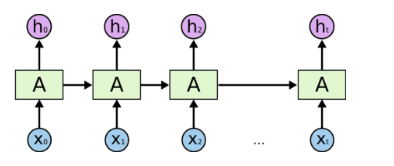
\includegraphics[width=3.5in]{../images/RNN}}
\centerline{{\large [Christopher Olah]}}
\vfill
Procedure $\mathrm{RNN}_\Phi(x(T,I))$

\vfill
\begin{eqnarray*}
h[t,J] & = & \mathrm{CELL}_{\Phi.\mathrm{cell}}(\mathrm{if}(t=0,\Phi.\mathrm{init}[J],h[t-1,J]),\;x[t,I]) \\
\end{eqnarray*}

\vfill
Return $h[T,J]$



\slide{bi-directional RNNS}

\centerline{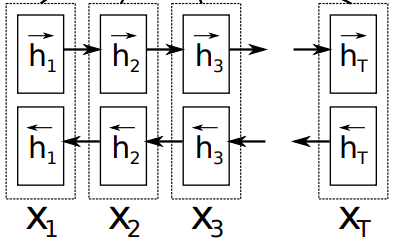
\includegraphics[width = 3in]{../images/biRNN}}

\begin{eqnarray*}
\vec{h}[T,\vec{J}] & = & \vec{\mathrm{RNN}}_{\Phi.LR}(x[T,I]) \\
\\
\cev{h}[T,\cev{J}] & = & \cev{\mathrm{RNN}}_{\Phi.RL}(x[T,I]) \\
\\
h[t,J] & = & [\vec{h}[T,\vec{J}],\;\cev{h}[t,\cev{J}]]\;\;\mbox{where $[x,y]$ is vector concatenation}
\end{eqnarray*}


\slide{Multi-Layer RNNs}

\centerline{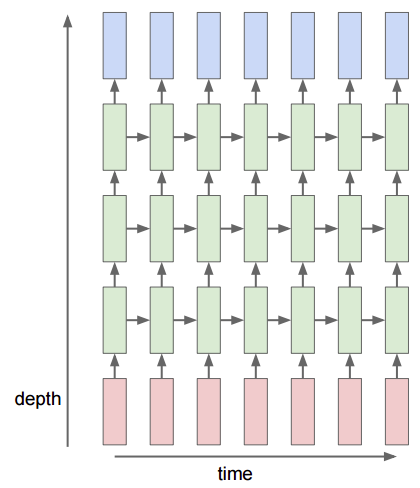
\includegraphics[width = 2in]{../images/RNNstack}}
\centerline{\large [Figure by Leonardo Araujo dos Santos]}

\begin{eqnarray*}
h[0,T,J] & = & \mathrm{RNN}_{\Phi.0}(x[T,I]) \\
\\
h[\ell+1,T,J] & = & \mathrm{RNN}_{\Phi.\ell+1}(h[\ell,T,J])
\end{eqnarray*}

Each layer can be bidirectional.

\anaslide{Residual Multi-Layer RNNs}

\begin{eqnarray*}
h[0,T,J] & = & \mathrm{RNN}_{\Phi.0}(x[T,I]) \\
\\
h[\ell+1,T,J] & = & h[\ell,T,J] + \mathrm{RNN}_{\Phi.\ell+1}(h[\ell,T,J])
\end{eqnarray*}

\vfill
Each layer can be bidirectional.

\vfill
This is used in Google translation.

\slide{ Language Modeling}

Let $W$ be some finite vocabulary of tokens (words).

\vfill
Let $\mathrm{Pop}$ be a population distribution over $W^*$ (sentences).

\vfill
We will write a sequence $w[1],\ldots,w[t]$ as $w[T]$.

\vfill
We want to train a model $P_\Phi(w[T])$.

\begin{eqnarray*}
\Phi^* & = & \argmin_\Phi \; E_{\mathrm{Pop}}\;-\ln P_\Phi(w[T])
\end{eqnarray*}

\slide{The End of Sentence Token}

\vfill
We assume a special toeken {\tt <EOS>} called the end of sentence token.

\vfill
Let $t_{\mathrm{final}}$ be the last time index allowed for $T$.

\vfill
We requite $w[t_{\mathrm{final}}] = \mbox{\tt <EOS>}$ and $w[t] \not = \mbox{\tt <EOS>}$ for $t < t_{\mathrm{final}}$.

\vfill
This gives:

$$P(w[T]) = \prod_t\;P(w[t]\;|\;w[1],\ldots,w[t-1])$$


\slide{Word Embeddings}

We will use a word embedding tensor $e[W,I]$ which should be interpreted as assigning a vector $e[w,I]$ to each word $w$.

\vfill
The word embedding tensor $e[W,I]$ is a parameter of language models (and many other kinds of NLP models).

\slide{Autoregressive Language Modeling}

Procedure $P_\Phi(w[T])$

\vfill
{\huge \begin{eqnarray*}
x[t,I] & = & (\Phi.\mathrm{embed})[w[t],I] \\
\\
h[T,J] & = & \mathrm{RNN}_{\Phi.\mathrm{RNN}}(x[T,I]) \\
\\
s[t,w] & = & \sum_{i,j} (\Phi.\mathrm{embed})[w,i]\;\;(\Phi.\mathrm{score})[i,j]\;\;\mathrm{if}(t=0,\Phi.\mathrm{init}[j],h[t-1,j]) \\
\\
p[t,w] & = & \softmax_w\;s[t,w]
\end{eqnarray*}
}

\vfill
Return $\prod_t p[t,w[t]]$

\slide{Language Model Loss Decomposition}

\begin{eqnarray*}
\Phi^* &  = & \argmin_\Phi\; E_{\mathrm{Pop}} \;-\ln\;P_\Phi(w[T]) \\
\\
\\
\\
& = & \argmin_\Phi\;E_{\mathrm{Pop}}\;\sum_t\; -\ln\;p[t,w[t]]
\end{eqnarray*}

\slide{Standard Measures of Performance}

{\bf Bits per Character:}
For character language models performance is measured in bits per character.  Typical numbers are slightly over one bit per character.

\vfill
{\bf Perplexity:}
It would be natural to measure word language models in bits per word.  However, it is traditional to measure then in perplexity which is defined to be
$2^b$ where $b$ is bits per word.  Perplexities of about 60 are typical.

\vfill
According to Quora there are 4.79 letters per word.  1 bit per character (including space characters) gives a perplexity of $2^{5.79}$ or $55.3$.

\slide{Sampling From an Autoregressive Model}

To sample a sentence
\vfill
$$w_1,\ldots, w_T, \mbox{\tt <eos>}$$
\vfill
we sample $w_t$ from
\vfill
$$P_\Phi(w_t|w_1,\ldots,w_{t-1})$$

\vfill
until we get {\tt <eos>}.


\slide{Machine Translation}

%\centerline{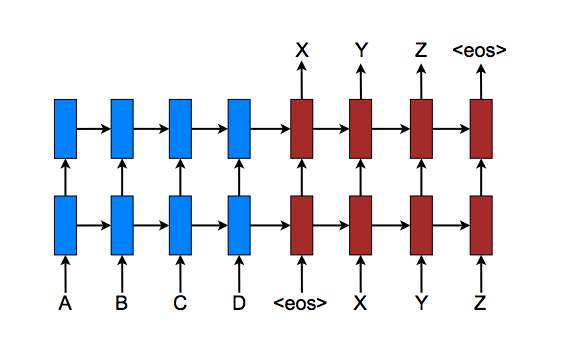
\includegraphics[width = 4in]{../images/SeqToSeq}}

%\centerline{\large [Figure from Luong et al.]}

$$w^{\mathrm{in}}_1,\ldots,w^{\mathrm{in}}_{t_{\mathrm{in}}} \Rightarrow w^{\mathrm{out}}_1,\ldots,w^{\mathrm{out}}_{t_{\mathrm{out}}}$$

$$w_{\mathrm{in}}[T_{\mathrm{in}}] \Rightarrow w_{\mathrm{out}}[T_{\mathrm{out}}]$$
\vfill
Translation is a {\bf sequence to sequence} (seq2seq) task.

\vfill
{\bf Sequence to Sequence Learning with Neural Networks}, Sutskever, Vinyals and Le, NIPS 2014, arXiv Sept 10, 2014.

\slide{Machine Translation}

%\centerline{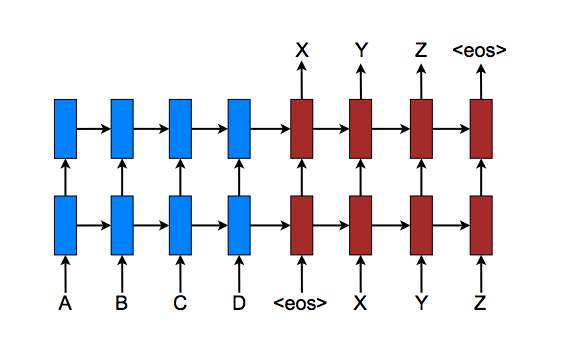
\includegraphics[width = 4in]{../images/SeqToSeq}}

%\centerline{\large [Figure from Luong et al.]}

$$w_{\mathrm{in}}[T_{\mathrm{in}}] \Rightarrow w_{\mathrm{out}}[T_{\mathrm{out}}]$$

\vfill
We define a model

\vfill
$$P_\Phi\left(w_{\mathrm{out}}[T_{\mathrm{out}}]\;|\; w_{\mathrm{in}}[T_\mathrm{in}]\right)$$

\vfill
\begin{eqnarray*}
\Phi^*  & = & \argmin_\Phi\; E_{\mathrm{Pop}} \;-\ln\;P_\Phi(w_{\mathrm{out}}[T_{\mathrm{out}}] \;|\; w_{\mathrm{in}}[T_{\mathrm{in}}]) \\
\\
& = & \argmin_\Phi \; E_{\mathrm{Pop}} \; -\ln P_\Phi(y|x)
\end{eqnarray*}


\slide{A Simple RNN Translation Model}

\vfill
We construct a conditional languge model

$$P_\Phi(w_{\mathrm{out}}[T_{\mathrm{out}}]\; | \; w_{\mathrm{in}}[T_{\mathrm{in}}]) = P_{\Phi.\mathrm{out}}(w_{\mathrm{out}}[T_{\mathrm{out}}] \;|\; H_{\Phi.\mathrm{in}}(w_{\mathrm{in}}[T_{\mathrm{in}}]))$$

\vfill
Here $H_{\Phi.\mathrm{in}}(w_{\mathrm{in}}[T_{\mathrm{in}}])$ is used as the initial hidden state of an RNN lnguage model.

\vfill
The initial hidden state $H_{\Phi.\mathrm{in}}(w_{\mathrm{in}}[T_{\mathrm{in}}])$ is a ``thought vector'' representation of the input sentence.

\slide{Computing a Thought Vector}

The thought vector for a sentence can be taken to be the final hidden state of a right-to-left RRN run on the sentence.

\vfill
Procedure $H_\Phi(w[T])$

\bigskip
$~\hspace{2em}\cev{h}[T,J] = \cev{\mathrm{RNN}}_\Phi\left(w[T]\right)$

\bigskip
Return $\cev{h}[t_{\mathrm{init}},J]$

\vfill
For a bidirectional RNN the thought vector is typically
\bigskip
$$\left[\cev{h}_{\mathrm{in}}[t_{\mathrm{init}},\cev{J}],\;\vec{h}_{\mathrm{in}}[t_{\mathrm{final}},\vec{J}]\right]$$

\slide{A Conditional RNN Language Modeling}

Procedure $P_\Phi(w[T] \;|\; {\color{red} H[J]})$

\vfill
{\huge \begin{eqnarray*}
x[t,I] & = & (\Phi.\mathrm{embed})[w[t],I] \\
\\
h[T,J] & = & \mathrm{RNN}_{\Phi.\mathrm{RNN}}(x[T,I] \;|\;{\color{red} H[J]}) \\
\\
s[t,w] & = & \sum_{i,j} (\Phi.\mathrm{embed})[w,i]\;\;(\Phi.\mathrm{score})[i,j]\;\;\mathrm{if}(t=0, {\color{red} H[j]},h[t-1,j]) \\
\\
p[t,w] & = & \softmax_w\;s[t,w]
\end{eqnarray*}
}

\vfill
Return $\prod_t p[t,w[t]]$

\slide{A Conditional RNN}

\centerline{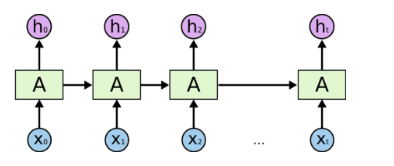
\includegraphics[width=3.5in]{../images/RNN}}
\centerline{{\large [Christopher Olah]}}
\vfill
Procedure $\mathrm{RNN}_\Phi(x(T,I)\;|\;{\color{red}H[J]})$

\vfill
\begin{eqnarray*}
h[t,J] & = & \mathrm{CELL}_\Phi(\mathrm{if}(t=0,{\color{red}H[J]},h[t-1,J]),\;x[t,I]) \\
\end{eqnarray*}

\vfill
Return $h[T,J]$

\slide{Machine Translation Decoding}

We can sample from $P_{\Phi.\mathrm{out}}(w[T]\;|\;H[J])$.

\vfill
But we might prefer

\begin{eqnarray*}
w_{\mathrm{out}}[T_{\mathrm{out}}]
& = & \argmax_{w_{\mathrm{out}}[T_{\mathrm{out}}]} \;P_\Phi\left(w_{\mathrm{out}}[T_{\mathrm{out}}] \;|\; w_{\mathrm{in}}[T_{\mathrm{in}}] \right)
\end{eqnarray*}

\vfill
This is typically approximated with greedy decoding:

\vfill
$$w_{\mathrm{out}}[t+1] = \argmax_w\; p_{\mathrm{out}}[t+1,w]$$

\vfill
These are not the same.



\slide{Attention-Based Translation}

\vfill
{\bf Neural Machine Translation by Jointly Learning to Align and Translate}
Dzmitry Bahdanau, Kyunghyun Cho, Yoshua Bengio, ICLR 2015 (arXiv Sept. 1, 2014)

\slide{Thought Vectors Augmented by Structed Memory}

The input sentence is now represented by both a thought vector and structured memory (a sequence of vectors).

\vfill
\begin{eqnarray*}
 & & P_\Phi(w_{\mathrm{out}}[T_{\mathrm{out}}] \;|\; w_{\mathrm{in}}[T_{\mathrm{in}}]) \\
 \\
& = & P_{\Phi.\mathrm{out}}(w_{\mathrm{out}}[T_{\mathrm{out}}]\;|\;
{\color{red} H_{\Phi.H}(w_{\mathrm{in}}[T_{\mathrm{in}}]),\;\mathrm{RNN}_{\Phi.\mathrm{RNN}}(w_{\mathrm{in}}[T_{\mathrm{in}}])})
\end{eqnarray*}

\slide{Attention-Based Translation}

Procedure $P_\Phi(w[T] \;|\; H[J],\;{\color{red} M[T_M,J]})$

\vfill
{\huge \begin{eqnarray*}
x[t,I] & = & (\Phi.\mathrm{embed})[w[t],I] \\
\\
h[T,J] & = & \mathrm{RNN}_{\Phi.\mathrm{RNN}}(x[T,I] \;|\;H[J],\;{\color{red} M[T_M,J]}) \\        
\\
s[t,w] & = & \sum_{i,j} (\Phi.\mathrm{embed})[w,i]\;\;(\Phi.\mathrm{score})[i,j]\;\;\mathrm{if}(t=0,\;H[j],\;h[t-1,j]) \\
\\
p[t,w] & = & \softmax_w\;s[t,w]
\end{eqnarray*}
}

\vfill
Return $\prod_t\;p[t,w[t]]$

\slide{Attention-Based Conditional RNN}

Procedure $\mathrm{RNN}_\Phi(x[T_x,I] \;|\; H[J],\; {\color{red} M[T_M,J]})$

\vfill
\begin{eqnarray*}
h[t,J] & = & \left\{\begin{array}{l}
\mathrm{CELL}_\Phi(H[J],[x[t,I],{\color{red}\mathrm{Val}(H[J],M[T,J])}]) \;\mbox{if $t = t_{\mathrm{init}}$} \\
\\
\mathrm{CELL}_\Phi(h[t-1,J],[x[t,I],{\color{red}\mathrm{Val}(h[t-1,J],M[T,J])}])\;\mbox{o.w.} \\
\end{array}\right.
\end{eqnarray*}

\vfill
Return $h[T,J]$

\slide{Attention as a Key-Value Memory Mechanism}

Procedure $\mathrm{Val}(\mathrm{key}[J],\;M[T,J])$

\bigskip
\begin{eqnarray*}
s[t] & = &\mathrm{key}[J]^\top M[t,J] \\
\\
{\color{red} \alpha[t]} & {\color{red} =} & {\color{red} \softmax_t \;s[t]\;\mbox{; the attention}} \\
\\
V[J] &= & \sum_t\;\alpha[t]M[t,J]
\end{eqnarray*}

\bigskip
Return $V[J]$



\slideplain{Attention in Image Captioning}

\centerline{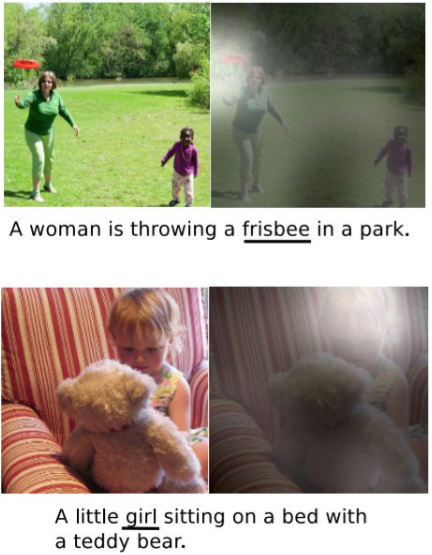
\includegraphics[width = 4in]{../images/AttentionInCaptioning1}}
\centerline{Xu et al. ICML 2015}

\slideplain{Greedy Decoding vs. Beam Search}

We would like

\vfill
$$W_{\mathrm{out}}[T_{\mathrm{out}}]^* = \argmax_{W_{\mathrm{out}}[T_{\mathrm{out}}]}
P_\Phi(W_{\mathrm{out}}[T_{\mathrm{out}}] \;|\;W_{\mathrm{in}}[T_{\mathrm{in}}])$$

\vfill
But a greedy algorithm may do well

\vfill
$$w_t = \argmax_w\; P_\Phi(w\;|\;W_{\mathrm{in}}[T_{\mathrm{in}}],\;w_1,\ldots,w_{t-1})$$

\vfill
But these are not the same.

\slide{Example}

``Those apples are good'' vs. ``Apples are good''

\vfill
$$P_\Phi(\mbox{Apples are Good {\tt <eos>}}) > P_\Phi(\mbox{Those apples are good {\tt <eos>}})$$

\vfill
$$P_\Phi(\mbox{Those}|\varepsilon) > P_\Phi(\mbox{Apples}|\varepsilon)$$
    
\slide{Beam Search}

At each time step we maintain a list the $K$ best words and their associated hidden vectors.

\vfill
This can be used to produce a list of $k$ ``best'' decodings which can then be compared to select
the most likely one.

\slideplain{Phrase Based Statistical Machine Translation (SMT)}

Step I:   Learn a phrase table --- a set of triples $(p,q,s)$ where

\vfill
\begin{itemize}
\item $p$ is a (short) sequence of source words.
  \vfill
\item $q$ is a (short) sequence of target words.
  \vfill
\item $s$ is a score.
\end{itemize}

\vfill
(``au'', ``to the'', .5) \hfill (``au banque'', ``for the bank'', .01)

\vfill
For a phrase triple $P$ we will write $P.\mathrm{source}$ for the source phrase, $P.\mathrm{target}$ for the target phrase, and $P.\mathrm{score}$ for the score.

\slide{Derivations}

Consider an input sentence $x$ of length $T$.

\vfill
We will write $x[s:t]$ for the substring $x[s]$, $\ldots$, $x[t-1]$.

\vfill
A derivation $d$ from $x$ is a sequence $(P_1,s_1,t_1,)$, $\ldots$, $(P_K,s_K,t_K)$ where $P_k.\mathrm{source} = x[s_k:t_k]$.

\vfill
The substrings $x[s_k:t_k]$ should be disjoint and ``cover'' $x$.

\vfill
For $d = [(P_1,s_1,t_1,)$, $\ldots$, $(P_L,s_K,t_K)]$ we define

$$ y(d) \equiv P_1.\mathrm{target}\;\cdots P_K.\mathrm{target}$$

\vfill
We let $D(x)$ be the set of derivations from $x$.

\slide{Scoring}

For $d \in D(x)$ we define a score $s(d)$

\vfill
$$s(d) = \alpha \ln P_\mathrm{LM}(y(d)) + \beta \sum_k P_k.\mathrm{score} + \gamma \;\mathrm{distortion}(d)$$

\vfill
where $P_{\mathrm{LM}}(y)$ is the probability assigned to string $y$ under a language model for the target language

\vfill
and $\mathrm{distortion}(d)$ is a measure of consistency of word ordering between source and target strings as defined by
the indeces $(s_1,t_1)$, $\ldots$, $(s_K,t_K)$.

\slide{Translation}

\begin{eqnarray*}
  y(x) & = & y(d^*(x)) \\
  \\
  \\
  \\
  d^*(x) & = & \argmax_{d \in D(x)} \;s(d)
\end{eqnarray*}

\slide{END}
}
\end{document}
